\documentclass[a4paper,10pt,twocolumn]{article}

% -------------------------------------------------
% PACOTES BÁSICOS
% -------------------------------------------------
\usepackage[utf8]{inputenc}
\usepackage[T1]{fontenc}
\usepackage[brazilian]{babel}

\usepackage[
    a4paper,
    top=2cm,
    bottom=3cm,
    left=2cm,
    right=2cm,
    footskip=0.8cm
]{geometry}

\usepackage{graphicx}
\usepackage{float}
\usepackage{placeins}
\usepackage{caption}
\usepackage[table]{xcolor}
\usepackage{fancyhdr}
\usepackage{helvet}
\usepackage{titlesec}
\usepackage{paracol}
\usepackage{indentfirst}
\usepackage{ragged2e}
\usepackage{hyperref}
\usepackage{csquotes}
\usepackage{newtxtext,newtxmath}
\usepackage{booktabs}
\usepackage{microtype}
\usepackage{enumitem}

% SVG
\usepackage{svg}

% Código
\usepackage{listings}
\usepackage{courier}

% -------------------------------------------------
% AJUSTES DE LAYOUT
% -------------------------------------------------

% Evita esticamento vertical exagerado
\raggedbottom

% Parâmetros permissivos para figuras
\renewcommand{\topfraction}{0.9}
\renewcommand{\bottomfraction}{0.8}
\renewcommand{\textfraction}{0.05}
\renewcommand{\floatpagefraction}{0.75}

% -------------------------------------------------
% DIAGRAMAS
% -------------------------------------------------
\usepackage{tikz}
\usetikzlibrary{shapes.geometric, arrows.meta, positioning}

% -------------------------------------------------
% BIBLIOGRAFIA
% -------------------------------------------------

\usepackage[
    backend=biber,
    style=ieee,
    sorting=none,
    language=portuguese
]{biblatex}

\addbibresource{referencias.bib}

% -------------------------------------------------
% CORES
% -------------------------------------------------
\definecolor{grayFEI}{HTML}{7F7F7F}
\definecolor{azulFEI}{HTML}{0070C0}

% -------------------------------------------------
% CONFIGURAÇÃO DO PACOTE LISTINGS PARA JSON
% -------------------------------------------------
\lstdefinelanguage{json}{
    basicstyle=\normalfont\ttfamily\footnotesize,
    showstringspaces=false,
    breaklines=true,
    stringstyle=\color{azulFEI},
    commentstyle=\color{grayFEI},
    keywordstyle=\bfseries
}

% -------------------------------------------------
% ESTILO DE PARÁGRAFOS
% -------------------------------------------------
\setlength{\parindent}{2em}
\setlength{\columnsep}{20pt}

% -------------------------------------------------
% LEGENDAS
% -------------------------------------------------
\captionsetup[figure]{
  labelfont={color=azulFEI,bf,small,sf},
  textfont={small,sf},
  font=footnotesize,
  labelsep=period,
  name=Figura,
  justification=raggedright,
  singlelinecheck=false
}

\captionsetup[table]{
  labelfont={color=azulFEI,bf,small,sf},
  textfont={small,sf},
  font=footnotesize,
  labelsep=period,
  name=Tabela,
  justification=raggedright,
  singlelinecheck=false
}

% -------------------------------------------------
% SEÇÕES E SUBSEÇÕES
% -------------------------------------------------
\titleformat{\section}
  {\color{azulFEI}\normalfont\fontfamily{phv}\selectfont\bfseries\fontsize{11}{13}\selectfont}
  {\thesection.}{0.2em}{}
\renewcommand{\thesection}{\Roman{section}}
\titlespacing*{\section}{0pt}{10pt}{4pt}

\titleformat{\subsection}
  {\color{grayFEI}\normalfont\fontfamily{phv}\selectfont\itshape\fontsize{10}{12}\selectfont}
  {\thesubsection.}{0.2em}{}
\renewcommand{\thesubsection}{\Alph{subsection}}
\titlespacing*{\subsection}{0pt}{6pt}{3pt}

% -------------------------------------------------
% COMANDOS DO TEMPLATE
% -------------------------------------------------
\newcommand{\helvetfont}[1]{{\fontfamily{phv}\selectfont #1}}

\newcommand{\inovatitle}[1]{%
  \noindent{\fontsize{18}{20}\selectfont\helvetfont{\textbf{\textcolor{azulFEI}{#1}}}}\par\vspace{25pt}
}

\newcommand{\autores}[1]{%
  \helvetfont{\fontsize{11}{20}\selectfont\textbf{\textit{#1}}}\par
}

\newcommand{\orientador}[1]{%
  \helvetfont{\fontsize{11}{20}\selectfont\textbf{\textit{#1}}}\par
}

\newcommand{\filiacao}[1]{%
  \helvetfont{\fontsize{10}{20}\selectfont\textit{#1}}\par
}

\newcommand{\email}[1]{%
  \helvetfont{\fontsize{10}{20}\selectfont\textit{#1}}\par
}

\newcommand{\resumo}[1]{%
  \vspace{15pt}
  \noindent
  {\helvetfont{\fontsize{12}{20}\selectfont\textbf{\textcolor{azulFEI}{Resumo:}}}}\quad
  \justifying #1\par
  \vspace{6pt}
}

\newcommand{\keyword}[1]{%
  \noindent
  \helvetfont{\fontsize{12}{20}\selectfont\textbf{\textcolor{azulFEI}{Palavras-chaves:}}} #1
  \vspace{25pt}\par
}

\renewcommand{\thetable}{\Roman{table}}

% -------------------------------------------------
% CABEÇALHO E RODAPÉ
% -------------------------------------------------
\pagestyle{fancy}
\fancyhf{}
\renewcommand{\headrulewidth}{0.3pt}
\setlength{\headsep}{1cm}
\setlength{\headheight}{1.2cm}

\IfFileExists{logoinova.png}
  {\lhead{
\includegraphics[width=4.97cm,height=1cm]{logoinova.png}}}
  {\lhead{\helvetfont{INOVA FEI}}}

\rhead{\helvetfont{1\textsuperscript{o} semestre/2026}}

\lfoot{%
  \fontfamily{phv}\fontsize{8}{10}\selectfont
  Anais dos Trabalhos de Conclusão de Curso do Centro Universitário FEI, São Bernardo do Campo \\
  \vspace{-4pt}\rule{\textwidth}{0.4pt}
}

\rfoot{\fontfamily{phv}\fontsize{8}{10}\selectfont \thepage}

% -------------------------------------------------
% ESTILOS TIKZ
% -------------------------------------------------
\tikzset{
  block/.style={
    rectangle, draw=black, rounded corners, align=center,
    minimum width=3.3cm, minimum height=0.95cm, fill=white
  },
  smallblock/.style={
    rectangle, draw=black, rounded corners, align=center,
    minimum width=2.7cm, minimum height=0.85cm, fill=white
  },
  wideblock/.style={
    rectangle, draw=black, rounded corners, align=center,
    minimum width=4.2cm, minimum height=0.95cm, fill=white
  },
  arrow/.style={-{Latex[length=3mm]}, thick}
}

\newcommand{\figlocal}[3]{%
  \par\medskip
  \noindent\begin{minipage}{\columnwidth}
    \centering
    #1
    \captionof{figure}{#2}
    \label{#3}
  \end{minipage}
  \par\medskip
}
% -------------------------------------------------
% DOCUMENTO
% -------------------------------------------------
\begin{document}

\twocolumn[
\begin{@twocolumnfalse}

\raggedright

\inovatitle{Sistemas Compostos de IA: Otimização de Respostas em Benchmarks Objetivos por meio de Orquestração Baseada no Ralph Loop}

\autores{Hugo Emílio Nomura, Pedro Henrique Correia de Oliveira, Pedro Henrique Satoru Lima Takahashi, Vitor Monteiro Vianna}

\filiacao{Ciência da Computação -- Centro Universitário FEI, campus São Paulo}

\email{unifhnomura@fei.edu.br, unifpoliveira@fei.edu.br, unifptakahashi@fei.edu.br, unievvianna@fei.edu.br}

\orientador{Orientador: Charles Henrique Porto Ferreira}

\filiacao{Departamento de Ciência da Computação, Centro Universitário FEI}

\email{cferreira@fei.edu.br}

\resumo{Embora os \textit{Large Language Models} (LLMs) continuem operando como geradores de texto, sua evolução recente não depende apenas do aumento de capacidade ou da complexidade matemática. Soluções modernas incorporam planejamento, refinamento e ciclos iterativos de raciocínio para melhorar a qualidade e a consistência das saídas. No entanto, o uso prolongado desses mecanismos amplia a janela de contexto e pode causar degradação de informação (\textit{context rot}), reduzindo a confiabilidade das respostas.

Este trabalho propõe adaptar os princípios do Ralph Wiggum Loop para cenários gerais de \textit{benchmarking}, com o objetivo de melhorar respostas por meio de chamadas iterativas ao próprio modelo, sem ferramentas externas. Para mitigar o \textit{context rot}, a arquitetura preserva um comportamento \textit{stateless} entre as fases, mantendo apenas os artefatos estritamente necessários a cada etapa.

O impacto empírico da abordagem será avaliado com os \textit{benchmarks} MMLU e GPQA, comparando a acurácia de chamadas diretas ao modelo com a de execuções mediadas pelo \textit{harness} proposto.}

\keyword{\textit{Large Language Models} (LLMs). Ralph Wiggum Loop. Sistemas Compostos de IA. Engenharia de Prompt. Decaimento de Contexto (\textit{context rot}).}

\end{@twocolumnfalse}
]

% =================================================
\section{Introdução}
% =================================================

Os \textit{Large Language Models} (LLMs) consolidaram-se como o núcleo de uma nova geração de sistemas capazes de executar tarefas complexas de processamento de linguagem natural, incluindo geração de texto, resolução de problemas, planejamento intermediário e suporte à tomada de decisão. Apesar dessas capacidades, os modelos que servem como base para esses sistemas continuam sendo, em essência, geradores probabilísticos de \textit{tokens}, operando a partir de uma entrada de texto e retornando como saída outro texto. Nesse contexto, parte significativa da evolução recente dos sistemas baseados em LLMs passou a ocorrer não apenas nos próprios modelos, mas também nas estruturas responsáveis por organizar sua utilização prática. Trabalhos recentes, como ~\cite{lee2026metaharness}, afirmam que \textit{``The performance of large language model (LLM) systems depends not only on model weights, but also on their harness: the code that determines what information to store, retrieve, and present to the model''}, evidenciando o papel dos chamados \textit{harnesses} na ampliação das capacidades desses sistemas. Ferramentas modernas, como o \textit{ChatGPT}, incorporam tais mecanismos para adicionar camadas de coordenação, decomposição de tarefas, validação intermediária e orquestração de múltiplas inferências, permitindo que o modelo execute fluxos significativamente mais sofisticados do que uma única chamada linear de entrada e saída.

Abordagens baseadas em uma única chamada ao modelo, nas quais toda a resposta é produzida em uma única etapa de inferência, apresentam limitações importantes em tarefas que exigem raciocínio complexo, múltiplas etapas de decisão ou validações intermediárias. Como resposta a esse problema, diferentes linhas de pesquisa passaram a explorar fluxos estruturados de \textit{thinking}, nos quais o processo de inferência é explicitamente decomposto em etapas sucessivas de raciocínio, planejamento, execução e refinamento. Trabalhos baseados em \textit{Chain-of-Thought}~\cite{wei2022chain}, \textit{Tree of Thoughts}~\cite{yao2023tree} e na técnica de \textit{Least-to-Most}~\cite{zhou2022least} demonstram que a decomposição explícita do raciocínio favorece significativamente a resolução de tarefas complexas. De maneira semelhante, abordagens como \textit{ReAct}~\cite{yao2022react} combinam raciocínio e ações iterativas, enquanto métodos como \textit{Reflexion}~\cite{shinn2023reflexion}, \textit{Self-Debugging}~\cite{chen2023selfdebug} e \textit{Self-Refine}~\cite{madaan2023selfrefine} exploram ciclos sucessivos de avaliação, crítica e refinamento da própria resposta gerada. Em conjunto, esses trabalhos indicam que ganhos de desempenho não dependem exclusivamente do tamanho do modelo ou da quantidade de \textit{tokens} gerados, mas também da maneira como o processo de inferência é estruturado, coordenado e validado ao longo da execução.

Apesar dos ganhos observados nessas arquiteturas iterativas compostas por agentes, ciclos de reflexão ou \textit{pipelines} sucessivos, tais abordagens também introduzem novos desafios relacionados ao gerenciamento do contexto acumulado durante a inferência. Em muitos desses sistemas, o histórico completo de interações permanece armazenado na janela de contexto ao longo de toda a execução como mecanismo de preservação da continuidade do raciocínio. Embora essa estratégia favoreça rastreabilidade e coerência entre etapas intermediárias, ela também aumenta progressivamente a dificuldade de recuperação de informações relevantes conforme o contexto cresce. Liu et al.~\cite{liu2023lost}, por exemplo, demonstram que ocorre perda de desempenho em tarefas que exigem localizar informações relevantes em sequências extensas. Trabalhos recentes também passaram a discutir fenômenos associados à degradação progressiva do contexto em execuções longas, incluindo compressão implícita de informações, perda de relevância contextual e aumento de inconsistências ao longo da inferência. Esses efeitos vêm sendo frequentemente associados, ao conceito de \textit{context rot}, termo utilizado por Hong et al.~\cite{hong2025context} para descrever a degradação gradual da qualidade das respostas conforme o volume de contexto acumulado aumenta.

Além do avanço acadêmico dessas abordagens, a indústria de engenharia de software também passou a investir intensamente em arquiteturas de \textit{deep thinking} e em \textit{harnesses} especializados para ampliar a capacidade operacional de LLMs em tarefas complexas de desenvolvimento. Ferramentas recentes, como \textit{Claude Code}, \textit{GPT Codex}, \textit{OpenCLI} e \textit{Devin}, exemplificam essa tendência ao combinar planejamento, decomposição de tarefas, validação iterativa e execução coordenada de múltiplas inferências. Nesse contexto, uma das abordagens que ganhou notoriedade foi o \textit{Ralph Wiggum Loop}~\cite{ghuntley2025ralph}, popularizado por Geoffrey Huntley no contexto de engenharia de software. Em sua formulação original, entretanto, o modelo não foi concebido para cenários generalistas, mas especificamente para fluxos de desenvolvimento baseados em conceitos próprios da engenharia de software, como definição de funcionalidades, requisitos, critérios de aceite e integração com sistemas de versionamento, como o \textit{Git}. Ainda assim, sua estrutura apresenta dois princípios centrais relevantes para os problemas discutidos na literatura de LLMs: a decomposição do processo em tarefas independentes, reduzindo a necessidade de reaproveitamento contínuo do contexto entre etapas, e a execução iterativa de cada tarefa até que critérios mínimos de qualidade sejam satisfatoriamente atingidos.

Este trabalho parte de três premissas consolidadas na literatura: que abordagens de \textit{thinking} podem melhorar a qualidade das respostas de LLMs em cenários específicos, como os de tarefas complexas; que tais abordagens introduzem problemas associados ao crescimento excessivo do contexto acumulado, fenômeno descrito como \textit{context rot}; e que o \textit{Ralph Wiggum Loop}~\cite{ghuntley2025ralph}, concebido por Huntley para fluxos de engenharia de software, oferece princípios estruturais capazes de mitigar o problema de \textit{context rot} por meio de decomposição de tarefas e isolamento contextual entre etapas. A partir dessas premissas, propõe-se a adaptação do \textit{Ralph Wiggum Loop} para um contexto generalista de resolução de tarefas em linguagem natural a partir de um \textit{prompt} de entrada fornecido pelo usuário. Diferentemente da proposta original, centrada em desenvolvimento de software, definições de funcionalidades, critérios de aceite baseados em requisitos funcionais e integração com ferramentas de versionamento (como Git), a adaptação proposta investiga se, ao adaptar a estrutura do \textit{Ralph Wiggum Loop} a um fluxo completo de \textit{thinking} aplicável à resolução de perguntas gerais e à exploração de problemas diversos e de diferentes complexidades, também haverá melhora na qualidade dessas respostas quando comparadas a uma única etapa de inferência.

Para avaliar essa hipótese de maneira objetiva, reproduzível e quantitativa, o trabalho compara diretamente duas estratégias de inferência: (i) uma chamada tradicional a um modelo de LLM, na qual toda a resposta é produzida em uma única etapa de inferência; e (ii) uma execução mediada pelo \textit{harness} proposto, que adapta o \textit{Ralph Wiggum Loop} para cenários generalistas. O objetivo experimental é medir em que magnitude a aplicação desse fluxo estruturado de \textit{thinking} melhora a qualidade das respostas em relação à inferência singular tradicional. Para permitir essa quantificação, os experimentos utilizam \textit{benchmarks} compostos por questões e respostas previamente definidas, estratégia amplamente adotada para mensuração de ganhos em arquiteturas de raciocínio e orquestração de LLMs, e usada em trabalhos como \textit{ReAct}~\cite{yao2022react} e \textit{Beyond the Strongest LLM}~\cite{wang2025beyond}. Os experimentos são conduzidos com diferentes modelos da família Llama 3.1, com diferentes quantidades de parâmetros utilizados na execução do modelo, representando distintos níveis de complexidade computacional, e avaliados por meio dos \textit{benchmarks} MMLU~\cite{hendrycks2021measuring} e GPQA~\cite{rein2023gpqa}, sendo a acurácia, medida pela quantidade de acertos entre a alternativa selecionada pelo sistema de LLM e o gabarito oficial.
% \FloatBarrier
% =================================================
\section{Referencial Bibliografico}
% =================================================

Esta seção apresenta os conceitos fundamentais necessários para a compreensão do trabalho proposto. São definidos os termos técnicos centrais utilizados ao longo do texto, descritas as principais estratégias de raciocínio e refinamento aplicadas a modelos de linguagem, e introduzido o paradigma de orquestração adotado neste trabalho.

\subsection{Modelos de Linguagem e a Arquitetura de Harness}

Embora os \textit{Large Language Models} (LLMs)~\cite{brown2020language} sejam amplamente consolidados como geradores probabilísticos de \textit{tokens} baseados na arquitetura \textit{Transformer}~\cite{vaswani2017attention}, a evolução recente na aplicação dessas tecnologias migrou de chamadas diretas e lineares para o uso de estruturas de orquestração mais robustas. Um detalhamento teórico e histórico aprofundado sobre o funcionamento desses modelos de linguagem pode ser encontrado no levantamento conduzido por Zhao et al.~\cite{zhao2023survey}.

Na prática, a organização dessas interações é viabilizada por meio de um \textit{harness}, termo que se refere à estrutura lógica e às regras de orquestração que envolvem um modelo de linguagem para guiar seu processo de inferência, funcionando como uma camada de coordenação entre o \textit{prompt} inicial do usuário e a saída do modelo~\cite{zaharia2024compound, wang2025beyond}. Um \textit{harness} pode incluir etapas de planejamento, decomposição de tarefas, validação intermediária e composição de respostas finais. Variações na arquitetura do \textit{harness} podem causar impactos significativos no desempenho do sistema como um todo, mesmo quando o modelo base permanece o mesmo.

Esse conceito está diretamente relacionado à noção de \textit{Sistemas Compostos de IA}, definida por Zaharia et al.~\cite{zaharia2024compound} como arquiteturas que resolvem tarefas de inteligência artificial por meio de múltiplos componentes que interagem entre si, incluindo chamadas a modelos, recuperadores de informação e ferramentas externas. Segundo essa perspectiva, os ganhos mais significativos em aplicações de IA contemporâneas passaram a depender da engenharia de sistemas que combinam componentes especializados em fluxos coordenados, em vez de se apoiarem unicamente no aumento de escala dos modelos base~\cite{zaharia2024compound}.

Essa tendência se manifesta em ferramentas industriais que utilizam LLMs integrados a \textit{harnesses} especializados para tarefas de engenharia e automação. Exemplos incluem o Claude Code~\cite{claudecode}, interface de linha de comando voltada ao desenvolvimento assistido por IA; o GPT Codex~\cite{chen2021evaluating}, otimizado para geração e compreensão de código; e o OpenCLI~\cite{opencli}, voltado à automação de comandos de terminal. Essas ferramentas demonstram como a combinação de planejamento, decomposição de tarefas e validação iterativa expande a capacidade computacional útil dos modelos base.

\subsection{Estratégias de Raciocínio e Refinamento}

A literatura demonstra que a qualidade da inferência de um LLM pode ser melhorada de forma significativa quando o processo é estruturado em fases~\cite{wei2022chain, yao2023tree}. O método \textit{Chain-of-Thought}~\cite{wei2022chain} e sua generalização \textit{Tree of Thoughts}~\cite{yao2023tree} mostraram a importância de induzir o modelo a explicitar passos intermediários de raciocínio. Abordagens como \textit{ReAct}~\cite{yao2022react} ampliaram esse princípio ao combinar o raciocínio interno do modelo com a capacidade de invocar ferramentas externas, permitindo corrigir alucinações por meio de observações diretas do ambiente.

De forma complementar, pipelines baseados em ciclos de \textit{feedback} iterativo também apresentam ganhos consistentes. O framework \textit{Reflexion}~\cite{shinn2023reflexion} introduziu ciclos nos quais o modelo atua como seu próprio crítico, revisando saídas com base em reforço verbal externo. A abordagem de \textit{Self-Debugging}~\cite{chen2023selfdebug} demonstrou que LLMs podem identificar e corrigir seus próprios erros quando guiados de forma sistemática. Na mesma direção, o método \textit{Self-Refine}~\cite{madaan2023selfrefine} consolidou a eficácia do refinamento iterativo ao demonstrar que modelos podem gerar \textit{feedback} crítico sobre suas próprias respostas e utilizá-lo para melhorar as saídas de forma sucessiva, contornando limitações da geração em uma única etapa. Essa capacidade de autocrítica e revisão contínua constitui uma premissa fundamental para a proposta deste trabalho.

Além dessas abordagens, métodos focados na decomposição de tarefas complexas também contribuem para a redução de erros lógicos e omissões. Técnicas de \textit{prompting} baseadas em decomposição, como \textit{Least-to-Most} \cite{zhou2022least}, \textit{Decomposed Prompting} \cite{khot2022decomposed} e \textit{Plan-and-Solve} \cite{wang2023plan}, sustentam que separar o planejamento da execução e dividir problemas em subproblemas menores melhora o desempenho do modelo, especialmente quando combinado com mecanismos de validação intermediária.

\subsection{Degradação de Contexto}


Embora as técnicas apresentadas nas subseções anteriores tenham demonstrado eficácia individual, muitas delas dependem do acúmulo contínuo de estado em uma única janela de contexto, o que pode agravar problemas de degradação à medida que o histórico cresce. Liu et al.~\cite{liu2023lost} demonstraram empiricamente que LLMs apresentam perda significativa de desempenho quando precisam recuperar informações relevantes posicionadas no meio de sequências longas, fenômeno descrito como ``perdidos no meio'' (\textit{lost in the middle}).

Na prática, esse comportamento se manifesta de diversas formas: compressão implícita de informações, perda de relevância contextual, aumento de inconsistências e maior incidência de alucinações em execuções prolongadas~\cite{liu2023lost, zhao2023survey}. A literatura contemporânea frequentemente associa esse conjunto de efeitos ao conceito de \textit{context rot}, referindo-se à degradação progressiva da qualidade das respostas conforme o contexto acumula ruído, redundâncias e informações que competem pela atenção do modelo~\cite{liu2023lost}.

\begin{figure*}[tb]
  \centering
  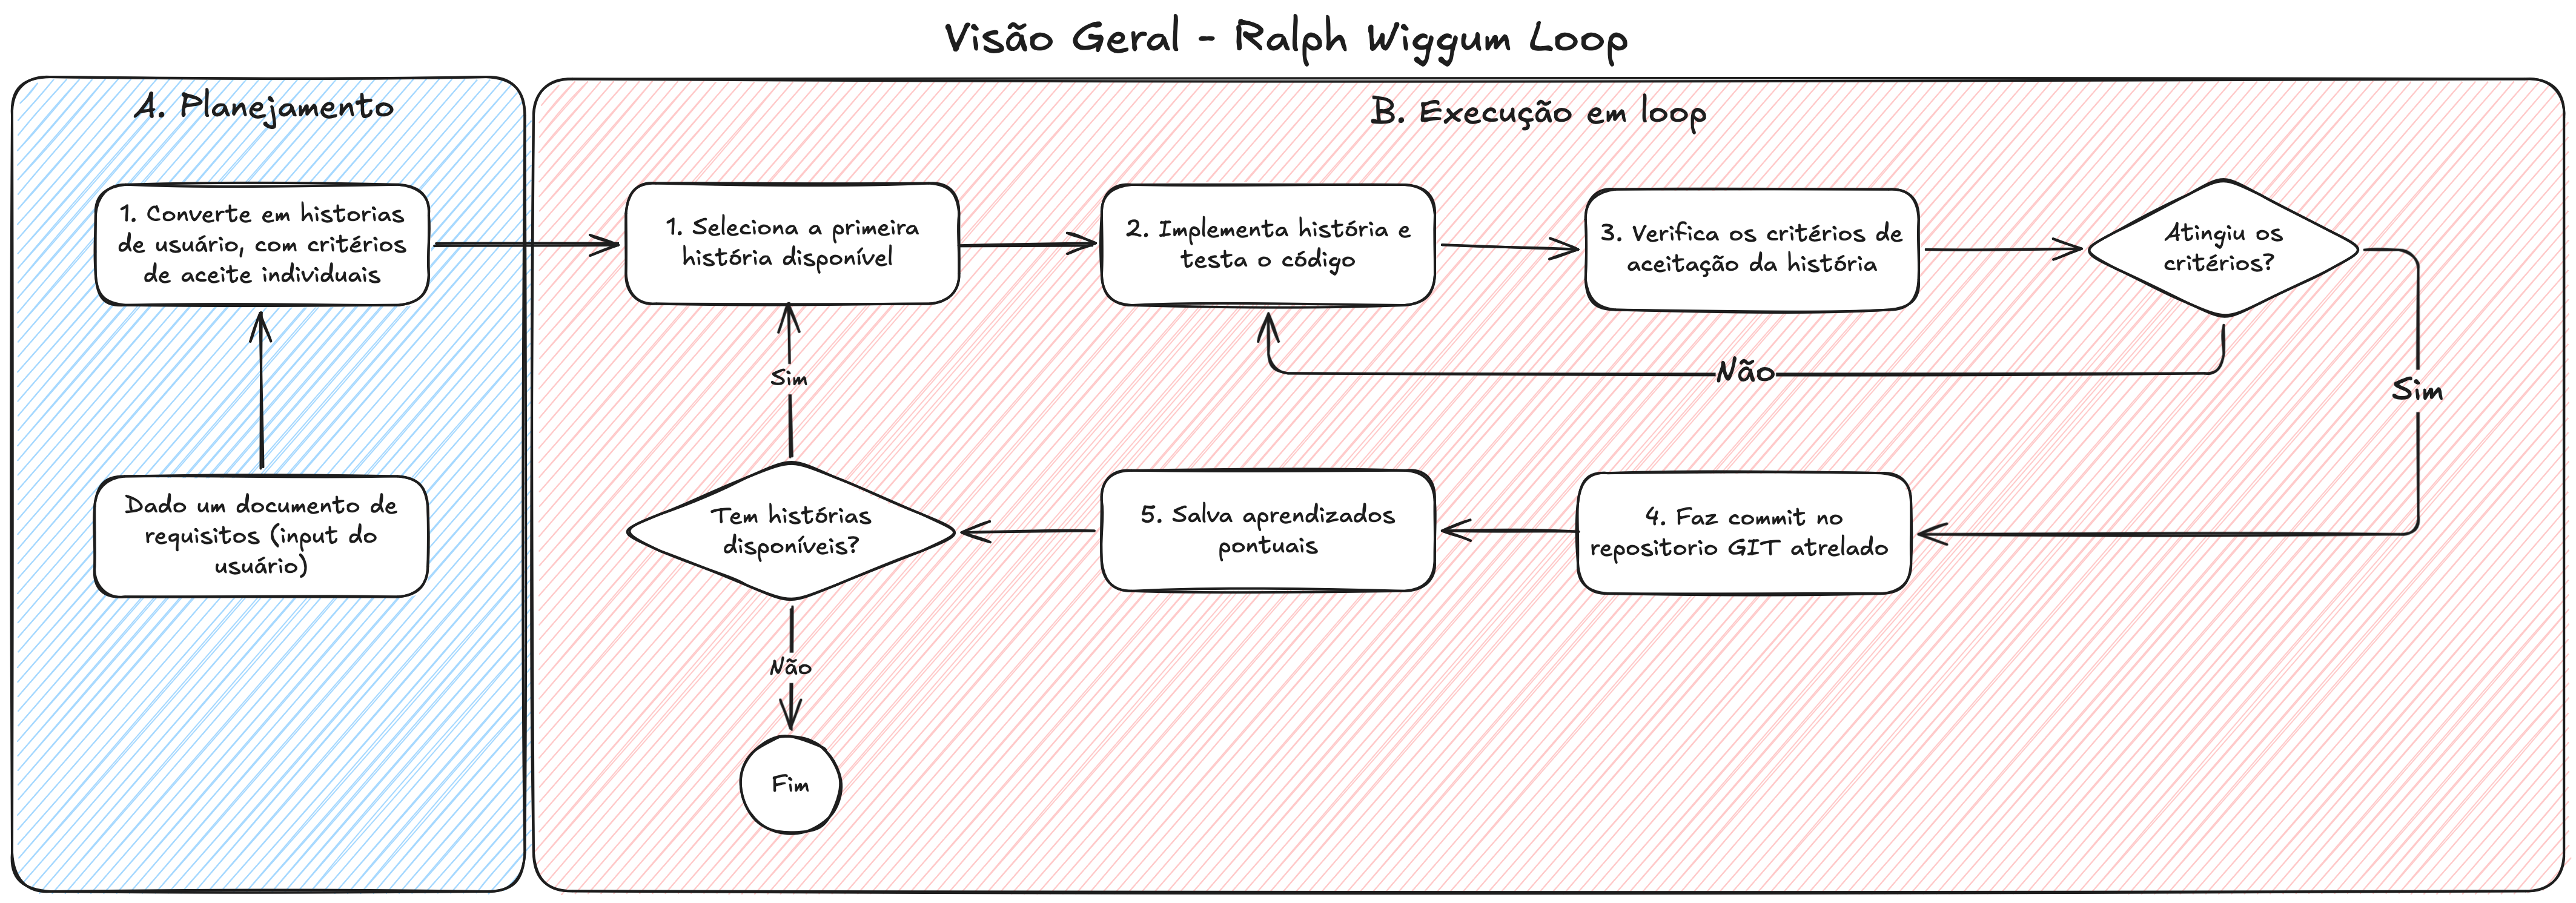
\includegraphics[width=\textwidth]{diagrams/ralph_loop_original_png}
  \caption{Ralph Wiggum Loop original.}
  \label{fig:ralph_loop_original}
\end{figure*}

\subsection{O Ralph Wiggum Loop}

Diante dos problemas de degradação de contexto, o \textit{Ralph Wiggum Loop}~\cite{ghuntley2025ralph} surgiu na comunidade de engenharia de software como um paradigma de orquestração que aborda diretamente essa limitação. Idealizado por Geoffrey Huntley, o paradigma parte de um conjunto de requisitos fornecidos como entrada e os decompõe em histórias de usuário, conceito consolidado na disciplina de engenharia de software. Cada história é tratada de forma atômica: o modelo implementa uma solução, executa testes e verifica se os critérios de aceite foram satisfeitos; caso contrário, o ciclo se repete até que a história seja concluída com êxito. Ao término de cada história, seus resultados não são carregados diretamente para a execução seguinte, evitando o acúmulo progressivo de estado que caracteriza arquiteturas tradicionais de agentes.

Um aspecto central dessa abordagem é o princípio de \textit{Fresh Context}~\cite{ghuntley2025ralph}: ao iniciar cada nova história, o contexto de execução é completamente reinicializado. Antes de qualquer instrução sobre a nova história, os aprendizados gerais extraídos das histórias anteriores são injetados como primeira entrada nesse novo contexto, de forma estruturada e explícita. Dessa maneira, o paradigma preserva o conhecimento relevante acumulado sem herdar o ruído, as redundâncias e as informações obsoletas que degradam progressivamente a qualidade das respostas em execuções longas, mitigando ativamente o fenômeno de \textit{context rot}~\cite{hong2025context}.

Em sua formulação original, o \textit{Ralph Wiggum Loop} foi concebido especificamente para fluxos de engenharia de software, com etapas voltadas à definição de funcionalidades, requisitos, critérios de aceite e integração com sistemas de versionamento como \textit{Git}. Ainda assim, seus princípios de execução \textit{stateless} e validação iterativa apresentam relevância direta para os problemas discutidos na literatura de LLMs. A validação acadêmica dessa abordagem foi reforçada pelo estudo de McComb et al.~\cite{supervising_ralph_wiggum_2026}, que avaliou o impacto de agentes baseados no \textit{Ralph Wiggum Loop} na resolução de problemas complexos de design de engenharia, confirmando a eficácia do paradigma \textit{stateless} em contextos que exigem raciocínio estruturado e iterativo. Este trabalho se apoia nesses fundamentos para justificar o uso do paradigma, adaptando sua orquestração para a resolução de questões de propósito geral em múltiplos domínios do conhecimento.


% =================================================
\section{Metodologia}
% =================================================

% \titleformat{\subsection}
%   {\color{grayFEI}\normalfont\fontfamily{phv}\selectfont\itshape\fontsize{10}{12}\selectfont}
%   {\arabic{subsection}.}        % Numeração arábica
%   {0.2em}
%   {}
% \renewcommand{\thesubsection}{\arabic{subsection}}  % Define arábica globalmente
% \titlespacing*{\subsection}{0pt}{6pt}{3pt}

\begin{figure*}[tb]
  \centering
  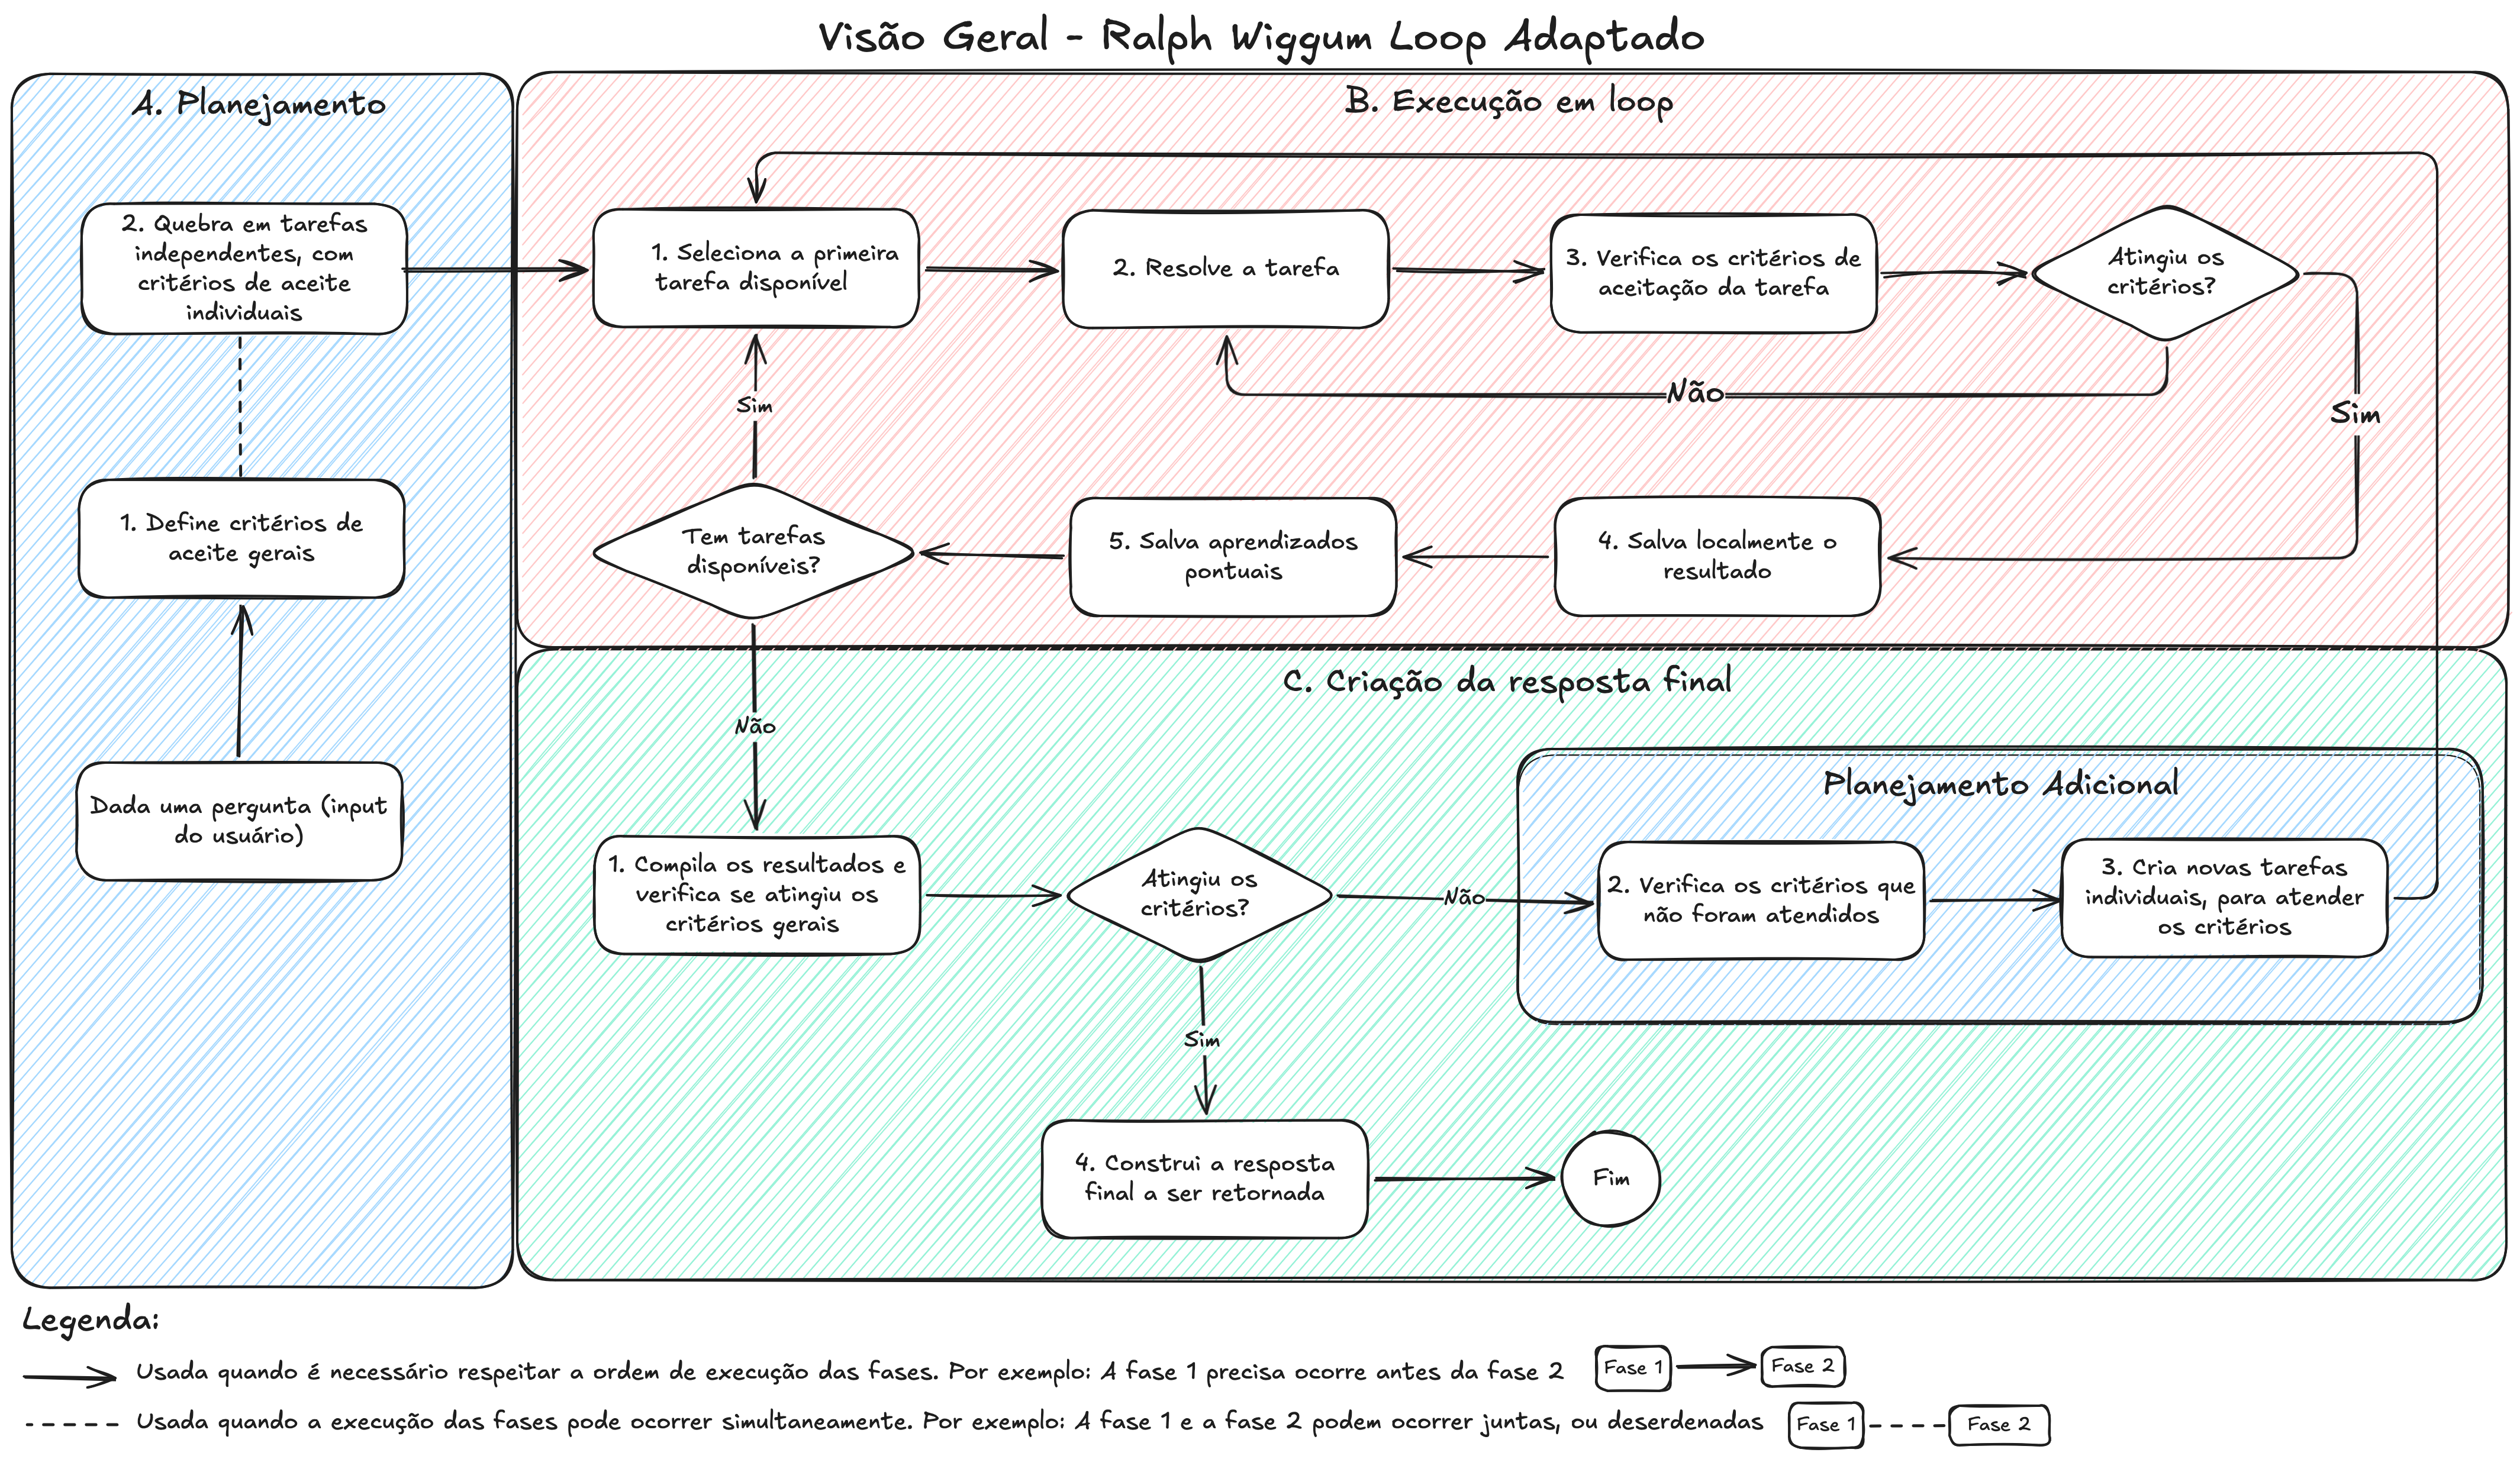
\includegraphics[width=\textwidth]{diagrams/ralph_loop_adaptado_png}
  \caption{Visão geral do \textit{Ralph Wiggum Loop} adaptado para resolução de perguntas em linguagem natural.}
  \label{fig:ralph_loop_adaptado}
\end{figure*}

A adaptação do \textit{Ralph Wiggum Loop} para um contexto generalista de resolução de perguntas em linguagem natural exige ajustes estruturais em relação à formulação original, que foi concebida exclusivamente para fluxos de engenharia de software. A Figura~\ref{fig:ralph_loop_adaptado} apresenta uma visão geral do fluxo proposto, que preserva os princípios centrais do paradigma original, representado na Figura~\ref{fig:ralph_loop_original}.

Em linhas gerais, propomos uma conversão do conceito de histórias de usuário para tarefas, o que nos permite manter um fluxo muito próximo do original, contendo as etapas de ``Planejamento'' e ``Execução em Loop''. Entretanto, passa a ser necessário considerar a criação de um retorno ao usuário, algo que não constitui uma preocupação no \textit{Ralph Wiggum Loop} original. Dessa forma, incorporamos uma nova fase após fluxo de execução, denominada ``Criação da Resposta Final'', que contém toda a lógica necessária para agrupar os resultados produzidos pelas tarefas anteriores em uma resposta que apresente o conteúdo e o formato esperados pelo usuário que realizou a solicitação.


% A. Planejamento
\subsection{Planejamento}

O planejamento é o inicio de todo o fluxo. Aqui assumimos que estamos recebendo uma pergunta e vamos iniciar o fluxo de \textit{Thinking} da aplicação. Assim como exemplificado na Figura~\ref{fig:ralph_loop_adaptado}, o planejamento possui somente duas etapas:

- Exemplo pratico de input passado pelo usuario:
\begin{quote}
Qual dos seguintes números é simultaneamente primo, par e maior que 2?

\begin{enumerate}[label=\Alph*)]
    \item 2
    \item 4
    \item 6
    \item Nenhuma das anteriores
\end{enumerate}
\end{quote}

\subsubsection{Defição dos critérios de aceite gerais}\label{subsec:planejamento-criterios}
- Explicação da responsabilidade:
  - Essa é uma fase que não era necessaria no contexto de desenvolvimento de software, ja que a cada tarefa que era entregue, um commit era feito salvando o progresso, e quando todas as terafas tivessem encerrado, o desenvolvimento tambemn estaria promto.
  - Agora o cenario muda, apos todas as tarefas serem todas concluidas, vai ser necessario enviar uma resposta final usando o resultado das tarefas geradas, e esses criterios devem trazer definições que vão ser usadas.
    - Vão ser definidos pontos como: Idioma a ser usado na resposta final, Qual o formato que deve ser construida a resposta final, topicos chaves do conteudo que devem estar presentes na resposta final

- Como vai ser feito:
  - Criação de um template FIXO, onde vai ser injetado o input passado pelo usuario. Esse template deve conter um prompt solicitando a definição de uma lista de criterios de aceite que vão ser resgatados na fase de criação da resposta final.
  - Deve ficar claro que o tempelate dessa fase vai somente pedir aquebra e fornecer exemplos dessas quebras
    - O template vai pedir para que ocorra definição de:
      - Idioma a ser usado na resposta final
      - Qual o formato que deve ser construida a resposta final
      - Topicos chaves do conteudo que devem estar presentes na resposta final

- Equação de funcinamento da fase:
  - Pergunta do usuario + Template A.1 = Resultado Fase A.1
  - O Resultado Fase A.1 deve ser armazenado localmente em um arquivo ou na memoria do programa

- Exmplo pratico:
  - Assumindo input passado no inicio o LLM deveria retornar algo como:
    - "A pergunta deve ser respondida em Portugues do Brasil", "Reponda somente a alternativa, sem conter explicações adicionais", "Garanta que o valor encontrado ao final bate com uma das alternativas"

\subsubsection{Quebra em tarefas de objetivo único com critérios de aceite individuais} \label{subsec:planejamento-tarefas}
- Explicação da responsabilidade:
  - Quebrar a pergunta do usuario em pequenas fases.
  - Cada fase precisa ter um criterio de aceite, ou seja, o conteudo que esperamos que seja gerado para que a fase possa ser considarada como "Concluida"
  - Aqui a ideia é criar fases que gerem insumos capazes de gerar uma resposta final ao se juntar.

- Como vai ser feito:
  - Criação de um template FIXO, onde vai ser injetado o input passado pelo usuario. Esse template deve conter um prompt solicitando a quebra da pergunta fornecida como input pelo ususario em tarefas.
    - Ainda nesse template, deve ser especificado que as tarefas de objetivo único, nesse contexto, significam ter uma unica responsabilidade pontual, como "pegar uma formula" ou "buscar o dado X", mas nunca "Buscar pela formula X, substituir pelos varelas A, B, C e executar a conta matemática para encontrar o resultado".
    - Alem de ter um unico objetivo, a terafa deve ser o mais detalhada possivel, para que não ocorram desvios de objetico.
    - Nesse prompt de quebra tambem deve ficar claro que o contexto doque foi feito não vai pra proxima fase, somente serão salvos pontos especificos que podem ser uteis para fases posteriores, como "A formula X é usada para calcular o consumo de energia elétrica"
    - Preciso que fique claro que o objetivo dessas fases é gerar insumos para que a a tarefa possa ser resolvida
    - Tambem nesse template deve ser definido que toda terafa deve ter pelo menos um criterio de aceite, que valida se a resposta final gerada contem o conteudo necessario para encerrar a fase

- Equação de funcinamento da fase:
  - Pergunta do usuario + Template A.2 = Resultado Fase A.2
    - O Resultado Fase A.2 deve ser armazenado localmente em um arquivo ou na memoria do programa

- Exmplo pratico:
  - Assumindo input passado no inicio o LLM deveria retornar algo como:
    "
  - Tarefa 1:
    - Tarefa:
      - "Dadas as opções (2, 4, 6), identifique quais desses números são primos"
    - Critérios de aceite:
      - "Deve retornar a lista de números primos encontrados nas alternativas."
      - "Deve incluir uma breve explicação da regra de identificação de números primos."
      - "A resposta não deve tentar resolver a questão final."
      - "A resposta não deve avaliar nenhuma outra condição"

  - Tarefa 2:
    - Tarefa:
      - "Dadas as opções (2, 4, 6), identifique quais desses números são pares"
    - Critérios de aceite:
      - "Deve retornar a lista de números pares encontrados nas alternativas."
      - "Deve incluir uma breve explicação da regra de identificação de números pares."
      - "A resposta não deve tentar resolver a questão final."
      - "A resposta não deve avaliar nenhuma outra condição"

  - Tarefa 3:
    - Tarefa:
      - "Dadas as opções (2, 4, 6), identifique quais desses números são estritamente maiores que 2."
    - Critérios de aceite:
      - "Deve retornar a lista de números maiores que 2 encontrados nas alternativas."
      - "Deve incluir uma breve justificativa matemática para a comparação estabelecida."
      - "A resposta não deve tentar resolver a questão final."
      - "A resposta não deve avaliar nenhuma outra condição"
    "

    - Nota. O formato usado é somente de exemplo para mostrar o conteudo que deve ser gerado ao fim



% B. Execução em Loop
\subsection{Execução em Loop}

A fase de execução preserva a estrutura iterativa do paradigma original, mas adapta o mecanismo de conclusão de cada unidade de trabalho. Na formulação original, a conclusão de uma história de usuário é verificada por meio da execução de testes automatizados e da análise dos critérios de aceite associados ao código produzido. No fluxo adaptado, como não há código a ser testado, o modelo simplesmente resolve a tarefa selecionada e, em seguida, verifica se o resultado satisfaz os critérios de aceite individuais definidos no planejamento. Caso os critérios não sejam atingidos, o modelo repete a resolução da mesma tarefa até que sejam satisfeitos.

Ao concluir uma tarefa com sucesso, o modelo salva o resultado localmente e registra os aprendizados pontuais obtidos ao longo daquela execução. Esses aprendizados correspondem ao mecanismo de \textit{Fresh Context} do paradigma original: antes de iniciar a execução da tarefa seguinte, o contexto é reinicializado e os aprendizados acumulados são injetados como primeira entrada do novo contexto, de forma estruturada e explícita. Esse mecanismo garante que o conhecimento relevante seja preservado sem que o ruído e as redundâncias das etapas anteriores sejam herdados, mitigando ativamente o fenômeno de \textit{context rot}~\cite{hong2025context}. Para o armazenamento local dos resultados, adota-se o formato JSON por conveniência de manipulação programática, embora qualquer formato que permita recuperação posterior seja funcionalmente equivalente. O ciclo se repete até que todas as tarefas planejadas sejam concluídas.


% C. Criação da Resposta Final
\subsection{Criação da Resposta Final}

A terceira fase constitui uma adição exclusiva do fluxo adaptado, sem correspondência direta na formulação original. No \textit{Ralph Wiggum Loop} concebido para engenharia de software, o produto final é o próprio código implementado e versionado ao longo das histórias; não há, portanto, necessidade de uma etapa de síntese posterior. No fluxo adaptado, os resultados das tarefas individuais são fragmentos de raciocínio que precisam ser compilados em uma resposta coesa e completa.

Após o encerramento do loop, o modelo compila os resultados armazenados e verifica se as informações produzidas são suficientes para satisfazer todos os critérios de aceite gerais definidos no planejamento. Se os critérios forem integralmente atendidos, o modelo constrói a resposta final e a retorna ao usuário. Caso contrário, o sistema infere que o planejamento inicial foi insuficiente para cobrir todos os aspectos da pergunta e inicia uma fase de \textit{Planejamento Adicional}: o modelo identifica os critérios ainda não atendidos, cria novas tarefas individuais para supri-los e retorna à fase de Execução em Loop. Esse mecanismo garante que lacunas de planejamento sejam identificadas e corrigidas antes que a resposta final seja construída, preservando a completude e a coerência da saída.







% -------------------------------------------------
\section{Cronograma do projeto}
% -------------------------------------------------

\begin{table*}[tb]
  \centering
  \caption{Cronograma das atividades do projeto.}
  \label{tab:cronograma}
  \renewcommand{\arraystretch}{1.2}
  \setlength{\tabcolsep}{4pt}
  \resizebox{\textwidth}{!}{%
  \begin{tabular}{|>{\columncolor{gray!15}}p{6.7cm}|*{10}{>{\centering\arraybackslash}p{0.72cm}|}}
    \hline
    \rowcolor{azulFEI!20}
    \textbf{Atividade} & \textbf{fev} & \textbf{mar} & \textbf{abr} & \textbf{mai} & \textbf{jun} & \textbf{jul} & \textbf{ago} & \textbf{set} & \textbf{out} & \textbf{nov} \\
    \hline
    Revisão bibliográfica e refinamento da proposta & X & X & X & X &  &  &  &  &  &  \\
    \hline
    Definição da arquitetura &  & X & X & X & X &  &  &  &  &  \\
    \hline
    Desenvolvimento do Paper &  & X & X & X & X & X & X & X & X & X \\
    \hline
    Implementação prática do código &  &  &  & X & X & X & X & X & X &  \\
    \hline
    Análise final &  &  &  &  &  &  &  &  & X & X \\
    \hline
  \end{tabular}%
  }
\end{table*}


% =================================================
\section{Referências}
% =================================================

\printbibliography

\end{document}
